\begin{figure}[H]
\centering
\caption{ The distributions of $\tau$ $\pt$ in the signal regions in leptonic channel. The samples shown in these figures are fake/real tau inclusive. In the rest of the plots in this note. The samples only includes real taus and the fake contribution are shown separately. Only statistical uncertainties are being shown. Underflow and overflow bins are included respectively in the first and last bins. Empty data bins here are always blinded based on our strategy.}

\includegraphics[page=6,width=0.48\textwidth]{\FCNCFigures/tthML/raw/faketau/prefit/NOMINAL/reg1l1tau1b1j_ss_vetobtagwp70_highmet/tau_pt_0.pdf}
%\put(-100, 140){\textbf{(a)}}
\put(-120, 130){\footnotesize{Fake/Real tau inclusive.}}
\includegraphics[page=6,width=0.48\textwidth]{\FCNCFigures/tthML/raw/faketau/prefit/NOMINAL/reg1l1tau1b2j_ss_vetobtagwp70_highmet/tau_pt_0.pdf}
%\put(-100, 140){\textbf{(b)}}
\put(-120, 130){\footnotesize{Fake/Real tau inclusive.}}

\includegraphics[page=6,width=0.48\textwidth]{\FCNCFigures/tthML/raw/faketau/prefit/NOMINAL/reg1l1tau1b2j_os_vetobtagwp70_highmet/tau_pt_0.pdf}
%\put(-100, 140){\textbf{(c)}}
\put(-120, 130){\footnotesize{Fake/Real tau inclusive.}}
\includegraphics[page=6,width=0.48\textwidth]{\FCNCFigures/tthML/raw/faketau/prefit/NOMINAL/reg1l1tau1b3j_os_vetobtagwp70_highmet/tau_pt_0.pdf}
%\put(-100, 140){\textbf{(d)}}
\put(-120, 130){\footnotesize{Fake/Real tau inclusive.}}

\includegraphics[page=6,width=0.48\textwidth]{\FCNCFigures/tthML/raw/faketau/prefit/NOMINAL/reg1l2tau1bnj_os/tau_pt_0.pdf}
%\put(-100, 140){\textbf{(e)}}
\put(-120, 130){\footnotesize{Fake/Real tau inclusive.}}
\label{fig:pt_raw}
\end{figure}
